\subsection{Ground station networks}

Ukjent nettverk
Ukjente deltakere
Ukjent utstyr

There are a lot of unknowns in this area. We don't know what network will be used, who will be participating or what kind of radio equipment will be used. In this section different networks have been simulated, see Table \ref{tab:networks}. 
Simulating a network consisting of NTNU and Aalborg University is interesting, since Aalborg University are the developers of the BlueBox satellite network.
\begin{figure}
  \begin{center}
    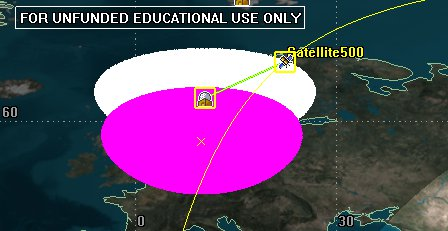
\includegraphics[width=0.7\textwidth]{Figures/range_ntnu_aalborg}
  \end{center}
  \caption[NTNU Aalborg]{Ground station network: NTNU and Aalborg}
  \label{fig:range_ntnu_aalborg}
\end{figure}

A ground station network consisting of NTNU and Aalborg University is not very efficent, see Fig. \ref{fig:range_ntnu_aalborg}. 
 
\begin{figure}
  \begin{center}
    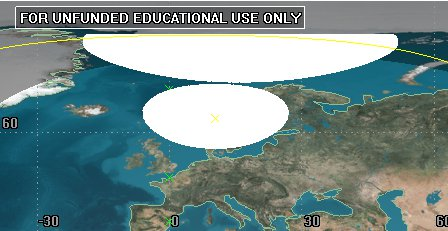
\includegraphics[width=0.7\textwidth]{Figures/range_ntnu_svalbard}
  \end{center}
  \caption[NTNU Aalborg]{Ground station network: NTNU and UNIS}
  \label{fig:range_ntnu_unis}
\end{figure}

\begin{table}
\begin{center}
\begin{tabular}{l | c c}
  Other locations & Time & Improvement \\
\hline \hline
  Aalborg & 790s &  50\% \\
\hline
  Longyearbyen & 1900s & 260\% \\
\hline
  Narvik & 900s & 73\%  \\
\end{tabular}
\end{center}
\caption{Some data}
\label{tab:networks}
\end{table}